\documentclass[11pt]{article}
\usepackage[T1]{fontenc}
\usepackage{lmodern}
\pdfglyphtounicode{parenleftbig}{0028}
\pdfglyphtounicode{parenrightbig}{0029}
\pdfglyphtounicode{parenleftBig}{0028}
\pdfglyphtounicode{parenrightBig}{0029}
\pdfgentounicode=1
\usepackage[margin=1.05in]{geometry}
\usepackage{amsmath,amssymb,amsthm,mathtools}
\usepackage{microtype}
\usepackage{enumitem}
\usepackage{xcolor}
\usepackage{tikz}
\usetikzlibrary{arrows.meta,positioning,calc}
\usepackage[hidelinks]{hyperref}
\hypersetup{pdftitle={A proof of Seymour's second-neighborhood conjecture},
 pdfsubject={Oriented graphs and finite relations}}
\pdftrailerid{}
\newtheorem{theorem}{Theorem}[section]
\newtheorem{lemma}[theorem]{Lemma}
\newtheorem{proposition}[theorem]{Proposition}
\newtheorem{corollary}[theorem]{Corollary}
\newtheorem{fact}[theorem]{Fact}
\theoremstyle{remark}
\newtheorem{remark}[theorem]{Remark}
\newtheorem{example}[theorem]{Example}
\newcommand{\abs}[1]{\lvert #1\rvert}
\DeclareMathOperator{\rank}{rank}
\DeclareMathOperator{\im}{im}
\newcommand{\R}{\mathbb R}
\newcommand{\unverified}[1]{\par\smallskip\noindent\fbox{\parbox{0.95\linewidth}{\textbf{Unverified step.} #1}}\par\smallskip}
\newcommand{\step}[1]{\par\medskip\noindent\textbf{Step #1.}\ }
\newcommand{\substep}[1]{\par\smallskip\noindent\textup{(#1)}\ }
\title{A proof of Seymour's second-neighborhood conjecture}
\author{Rewritten for readability from the OpenAI manuscript of the same title}
\date{September 23, 2026}
\begin{document}
\maketitle
\begin{abstract}
We prove that every nonempty finite oriented graph has a vertex with at least
as many vertices at directed distance two as at directed distance one.
This resolves Seymour's second neighborhood conjecture positively.
\end{abstract}

\section{The main result}\label{sec:introduction}

\paragraph{Setting.}
An \emph{oriented graph} is a finite directed graph with no loops, no multiple
arcs, and no pair of opposite arcs. Its underlying undirected graph need not
be complete or connected. We write $v\to u$ when there is an arc from $v$ to
$u$. For a vertex $v$ put
\[
 N_1^+(v)=\{u:v\to u\},\qquad
 N_2^+(v)=\{w\notin\{v\}\cup N_1^+(v):
                 \text{ there is a vertex }u\text{ with }v\to u\to w\}.
\]
Thus $N_2^+(v)$ is the set of vertices at directed distance exactly two from
$v$; each such vertex is counted once, however many paths reach it.

\begin{theorem}\label{thm:main}
Every nonempty finite oriented graph has a vertex \(v\) such that
\[
 \abs{N_1^+(v)}\leq \abs{N_2^+(v)}.
\]
\end{theorem}

There is no connectivity or degree hypothesis. Two sanity checks: a sink
($N_1^+(v)=\varnothing$) satisfies the conclusion trivially, and in a directed
triangle every vertex has $\abs{N_1^+(v)}=\abs{N_2^+(v)}=1$.

\paragraph{The image operator.}
For a digraph $D$ and a set $S\subseteq V(D)$ define
\[
 F_D(S)=\{y:\text{ there is }x\in S\text{ with }x\to y\},
 \qquad F_D^2(S)=F_D(F_D(S)).
\]
Note that $F_D$ does \emph{not} subtract $S$: $F_D(S)$ may meet $S$. We
drop the subscript when the graph is clear. The following elementary facts
are used throughout without further comment.

\begin{fact}\label{fact:image}
Let $D$ be a digraph and $A,B\subseteq V(D)$.
\begin{enumerate}[label=\textup{(\alph*)}]
\item $F(\varnothing)=\varnothing$, $F(A\cup B)=F(A)\cup F(B)$, and
$A\subseteq B$ implies $F(A)\subseteq F(B)$.
\item If $D'$ is obtained from $D$ by deleting arcs, then
$F_{D'}(A)\subseteq F_D(A)$ and $F_{D'}^2(A)\subseteq F_D^2(A)$.
\item $F(V(D))=V(D)$ if and only if every vertex has positive indegree.
\item If $D$ is oriented, then $N_1^+(v)=F(\{v\})$,
$v\notin F(\{v\})\cup F^2(\{v\})$, and
$N_2^+(v)=F^2(\{v\})\setminus F(\{v\})$.
\end{enumerate}
\end{fact}

\begin{proof}
(a)--(c) are immediate from the definition. For (d): $v\notin F(\{v\})$
because there are no loops, and $v\in F^2(\{v\})$ would give $v\to u\to v$,
a pair of opposite arcs. By definition
$N_2^+(v)=F^2(\{v\})\setminus(\{v\}\cup F(\{v\}))$, and removing $v$ changes
nothing since $v\notin F^2(\{v\})$.
\end{proof}

\paragraph{Consequences.}
Section~\ref{sec:weighted-consequences} derives vertex- and arc-weighted
forms of the theorem through Seacrest's equivalences~\cite{Seacrest2015}.
Section~\ref{sec:directed-cycle-consequences} records consequences for short
directed cycles. For example, an oriented graph with minimum in- and
outdegree at least one third of its order contains a directed triangle.

\section{Proof at a glance}\label{sec:glance}

The proof is by contradiction. It has two halves that are logically
independent and meet at one inequality. For an oriented graph $G$ consider
the \emph{strict concavity inequality}
\begin{equation}\label{eq:overview-concavity}
 \abs{U}+\abs{F_G^2(U)}<2\abs{F_G(U)}
 \qquad\text{for every }\varnothing\ne U\subsetneq V(G).
\end{equation}

\begin{itemize}[leftmargin=2em]
\item \textbf{Half A (Section~\ref{sec:reduction},
Proposition~\ref{prop:counterexample-reduction}).} If
Theorem~\ref{thm:main} fails, then some nonempty oriented graph $G$ with all
indegrees positive satisfies~\eqref{eq:overview-concavity}.
\item \textbf{Half B (Sections~\ref{sec:pruning}
and~\ref{sec:incompatibility}, Proposition~\ref{prop:no-concavity}).} No
nonempty oriented graph with all indegrees positive
satisfies~\eqref{eq:overview-concavity}.
\end{itemize}

\paragraph{Half A in two steps.}
\begin{enumerate}[label=\textbf{A\arabic*.},leftmargin=3em]
\item \emph{Subset deficit (Lemma~\ref{lem:subset-deficit}).} Take a
counterexample $D$ with the fewest vertices and then the fewest arcs. Then
every nonempty proper $S\subsetneq V(D)$ satisfies
$\abs{F^2(S)\setminus F(S)}<\abs{F(S)\setminus S}$. Idea: delete the arcs from
$S$ into part of $F(S)\setminus S$. By minimality some vertex $v$ of the
smaller graph satisfies the second-neighborhood inequality, and $v$ must have
lost a set $Q$ of out-neighbors. Comparing $v$ before and after the deletion
bounds the growth of a counting function by strictly less than $\abs Q$;
summing over a chain of such steps gives the deficit.
\item \emph{Blowup (Lemma~\ref{lem:blowup}).} Replace each vertex of $D$ by a
transitive tournament on $m>\abs{V(D)}$ vertices. The integer deficit of
step A1 is multiplied by $m$ and beats an error term of at most
$\abs{V(D)}$, which yields~\eqref{eq:overview-concavity}.
\end{enumerate}

\paragraph{Half B in three steps.}
\begin{enumerate}[label=\textbf{B\arabic*.},leftmargin=3em]
\item \emph{A rank fact (Lemma~\ref{lem:kernel-support}).} If a matrix has
maximum rank among matrices with a prescribed zero pattern, its left and right
kernels cannot both be nonzero at an allowed entry.
\item \emph{Pruning (Lemma~\ref{lem:pruning}).} Given two families
$\mathcal R,\mathcal C$ of ordered pairs and a ``conflict'' relation between
them, one can delete members to remove all conflicts, keeping every
conflict-free member, at a cost of at most $\abs H$ plus the number of points
of $Z$ left uncovered \emph{after} the deletion ($H$, $Z$ are two sets
determined by the conflicts). The proof finds a small vertex cover in an
auxiliary bipartite graph; by K\H{o}nig's theorem this reduces to bounding a
maximum matching by $\abs Z+\abs H$, which is done by comparing ranks of four
matrices satisfying $NL=AB$, using B1. This lemma holds for any finite binary
relation.
\item \emph{Extremal contradiction (Proposition~\ref{prop:no-concavity}).}
Work with pairs of families $P,Q\subseteq V(G)\times V(G)$ that contain the
diagonal and are \emph{compatible} (their coordinate images are disjoint).
Let $M=\abs P+\abs Q$ and let $d$ be the number of points in neither image;
choose $(P,Q)$ maximizing $M+d$. Applying~\eqref{eq:overview-concavity} to
the columns of $P$ and rows of $Q$ and passing to complements of second
images gives new families of total size $>M+2d$. They may conflict; pruning
(B2) repairs this at cost at most $d+d'$, where $d'$ is the new number of
uncovered points. The new objective is therefore
\[
 >\;M+2d-(d+d')+d'=M+d ,
\]
contradicting maximality. This is why the pruning cost must be charged partly
to points left uncovered after pruning, and why $d$ is part of the objective.
\end{enumerate}

\paragraph{Dependencies.}
\begin{center}
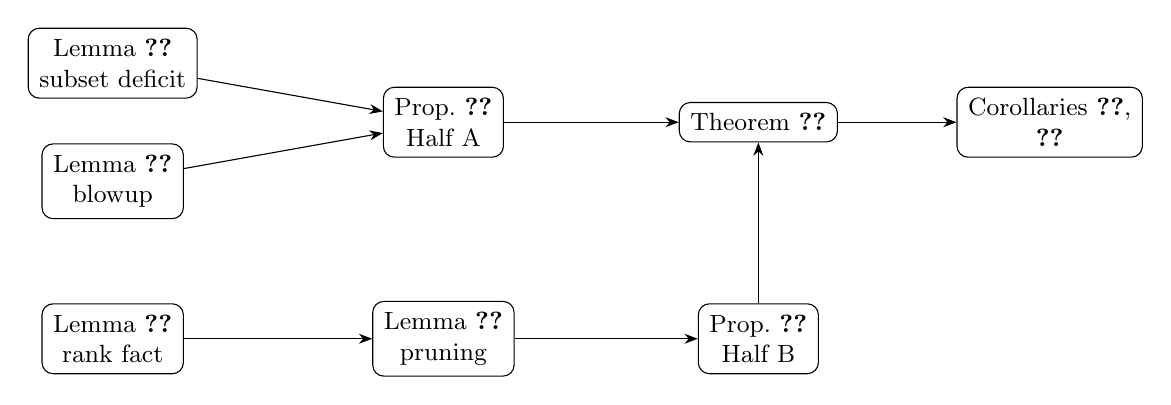
\begin{tikzpicture}[
  box/.style={draw,rounded corners,align=center,font=\small,inner sep=4pt},
  >={Stealth}]
 \node[box] (sd)  at (0,0.8)   {Lemma~\ref{lem:subset-deficit}\\ subset deficit};
 \node[box] (bl)  at (0,-0.7)  {Lemma~\ref{lem:blowup}\\ blowup};
 \node[box] (red) at (4.2,0.05) {Prop.~\ref{prop:counterexample-reduction}\\ Half A};
 \node[box] (ker) at (0,-2.7)  {Lemma~\ref{lem:kernel-support}\\ rank fact};
 \node[box] (pr)  at (4.2,-2.7) {Lemma~\ref{lem:pruning}\\ pruning};
 \node[box] (nc)  at (8.2,-2.7) {Prop.~\ref{prop:no-concavity}\\ Half B};
 \node[box] (thm) at (8.2,0.05) {Theorem~\ref{thm:main}};
 \node[box] (cor) at (11.9,0.05) {Corollaries~\ref{cor:weighted-forms},\\ \ref{cor:directed-cycle-consequences}};
 \draw[->] (sd) -- (red);
 \draw[->] (bl) -- (red);
 \draw[->] (red) -- (thm);
 \draw[->] (ker) -- (pr);
 \draw[->] (pr) -- (nc);
 \draw[->] (nc) -- (thm);
 \draw[->] (thm) -- (cor);
\end{tikzpicture}
\end{center}
Corollary~\ref{cor:weighted-forms} additionally uses two cited results of
\cite{Seacrest2015}.

\paragraph{Where orientation is used.}
The absence of opposite arcs enters through Fact~\ref{fact:image}(d) in
Lemma~\ref{lem:subset-deficit}, in checking that the blowup is oriented, and
in Proposition~\ref{prop:no-concavity} at exactly one place: the diagonal
families are compatible. Lemmas~\ref{lem:kernel-support}
and~\ref{lem:pruning} do not use it.

\paragraph{Notation and renamings.}
Letters introduced inside a proof are local to that proof. To avoid clashes
the following symbols differ from the source manuscript; nothing else is
changed.
\begin{itemize}[leftmargin=2em,itemsep=1pt]
\item The source's support-rank matrices $D$, $D^{p,i}$ and supports $T$,
$T^{p,i}$ (Section~\ref{sec:pruning}) are written $\Phi$, $\Phi^{p,i}$ and
$\Sigma$, $\Sigma^{p,i}$; $D$ is reserved for digraphs.
\item Label sets inside a block of the blowup are $\Lambda$, $\Lambda_v$
(source: $T$, $T_v$).
\item Summation indices over $R_\alpha$, $C_\beta$ are $\rho,\gamma$ (source:
$a,b$, which are also names of matrix coefficients).
\item A generic subset of $X\times X$ in Section~\ref{sec:incompatibility} is
$Y$ (source: $S$).
\item In Section~\ref{sec:weighted-consequences} the sign matrix is $\Psi_D$
(source: $M_D$), and in Section~\ref{sec:directed-cycle-consequences} the
non-neighbor set is $N^0(v)$ (source: $Z(v)$).
\item In Section~\ref{sec:pruning} the letters $u,v,x,y$ denote vectors;
elements of the ground set $X$ are called $p,i,s,j$ there.
\end{itemize}

\section{Context and prior work}\label{sec:context}

This section is not needed for the proof.

The conjecture was recorded by Dean and Latka~\cite{DeanLatka1995}.
A \emph{tournament} is an oriented graph with an arc between every pair of
distinct vertices. This case, also known as Dean's conjecture, was proved
by Fisher~\cite{Fisher1996} using a probability distribution obtained from
Farkas' lemma. Havet and Thomass\'e gave a combinatorial proof using
local median orders~\cite{HavetThomasse2000}. Fidler and
Yuster~\cite{FidlerYuster2007} extended the tournament theorem to
tournaments missing a matching, a star, or a clique. Ghazal corrected the
star-case proof and treated generalized stars~\cite{Ghazal2012}.
Subsequent advances include a matching together with a
star~\cite{DaraFrancisJacobNarayanan2022} and two
stars~\cite{DaamouchAlMninyGhazal2025}.

Other approaches impose degree conditions or weaken the desired ratio.
Kaneko and Locke established the conjecture for minimum outdegree at most
six~\cite{KanekoLocke2001}; a recent computer-assisted preprint treats
minimum outdegree seven~\cite{SadhukhanSandeepSen2026}.
Chen, Shen and Yuster proved a universal second-to-first neighborhood
ratio of approximately $0.657298$~\cite{ChenShenYuster2003}.
Huang and Peng raise this to approximately $0.715538$ and additionally
report a computational bound of $0.74530$~\cite{HuangPeng2024}.
Botler, Moura and Naia~\cite{BotlerMouraNaia2023}, followed by
Espuny D\'iaz, Gir\~ao, Granet and Kronenberg~\cite{EspunyDiazEtAl2025},
studied every orientation of binomial random graphs; the latter result
covers every fixed edge probability below $1/2$, with probability tending
to one as the order tends to infinity. Brukhman's recent dense-case
preprint concerns graphs of order $n\leq 2\delta+2$, where $\delta$ is
the minimum outdegree~\cite{Brukhman2026}.

The present proof builds on the minimal-counterexample and graph-product
methods of Brantner, Brockman, Kay and
Snively~\cite{BrantnerBrockmanKaySnively2009} and on Seacrest's
subset perspective~\cite{Seacrest2019}. The arc-deletion argument in
Lemma~\ref{lem:subset-deficit} adapts the proof idea of
\cite[Lemma~4]{Seacrest2019}. Specializing Seacrest's parameter $\lambda$
to $1$, his statement gives
$\abs{F^2(S)\setminus F(S)}<\abs{F(S)}$ in an edge-minimal
counterexample when $F(S)$ is nonempty; Lemma~\ref{lem:subset-deficit}
replaces this right-hand bound by $\abs{F(S)\setminus S}$ for nonempty
proper $S$, under the stronger choice of minimum order and then minimum
arc count, and is proved here in full. The blowup of Lemma~\ref{lem:blowup}
is the lexicographic product of $D$ with a transitive tournament; the same
construction appears in \cite[Theorem~4.3]{BrantnerBrockmanKaySnively2009},
but here an estimate is needed for every nonempty proper subset rather than
only for individual vertices. The main additional ingredient is the pruning
bound of Lemma~\ref{lem:pruning}.

\section{Half A: from a counterexample to strict concavity}
\label{sec:reduction}

\begin{proposition}[Counterexample reduction]
\label{prop:counterexample-reduction}
If Theorem~\ref{thm:main} has a counterexample, then there is a finite
nonempty oriented graph $G$ in which every vertex has positive indegree
and
\begin{equation}
\label{eq:strict-subset-growth}
  \abs{U}+\abs{F_G^2(U)}<2\abs{F_G(U)}
  \qquad\text{for every }\varnothing\ne U\subsetneq V(G).
\end{equation}
\end{proposition}

The proof is at the end of this section; it combines the next two lemmas.

\subsection{Subset deficit in a minimal counterexample}

The following lemma is used once, as the input to Lemma~\ref{lem:blowup}.
Throughout this subsection $F=F_D$.

\begin{lemma}[Subset deficit]
\label{lem:subset-deficit}
Let $D$ be a finite nonempty oriented graph such that
$\abs{N_1^+(v)}>\abs{N_2^+(v)}$ for every $v\in V(D)$.
Choose $D$ with minimum order and, subject to that, minimum number of
arcs among all graphs with this property. Then $D$ is strongly connected,
every vertex has positive indegree, and
\begin{equation}
\label{eq:subset-deficit}
  \abs{F^2(S)\setminus F(S)}<\abs{F(S)\setminus S}
  \qquad\text{for every }\varnothing\ne S\subsetneq V(D).
\end{equation}
\end{lemma}

\begin{proof}
Call a finite nonempty oriented graph \emph{bad} if
$\abs{N_1^+(v)}>\abs{N_2^+(v)}$ for all its vertices. So $D$ is bad, no bad
graph has fewer vertices, and no bad graph on $\abs{V(D)}$ vertices has fewer
arcs.

\emph{Plan.} Steps 1--3 give the structural claims. For a fixed $S$, we write
$E=F(S)\setminus S$ and define a counting function $g$ on subsets of $E$
with $g(\varnothing)=0$ and $g(E)=\abs{F^2(S)\setminus F(S)}$. Step~5 shows
that any $T\subsetneq E$ can be enlarged by a nonempty set $Q$ with
$g(T\cup Q)-g(T)<\abs Q$; Steps 6--7 sum these increments.

\step{1 ($D$ has no sink and at least two vertices)}
If $N_1^+(v)=\varnothing$ then $0>\abs{N_2^+(v)}$, which is impossible. So
every vertex has an out-neighbor, which is a different vertex since there are
no loops.

\step{2 ($D$ is strongly connected)}
The strong components of $D$ partition $V(D)$, and the digraph of components
is acyclic, so some strong component $K$ has no arc entering it. For $v\in K$
we get $N_1^+(v)\subseteq K$, and every path $v\to u\to w$ lies in $K$. Hence
$N_1^+(v)$ and $N_2^+(v)$ are the same whether computed in $D$ or in the
induced subgraph $D[K]$, so $D[K]$ is bad. By minimality of the order,
$K=V(D)$.

\step{3 (positive indegrees)}
Given a vertex $w$, pick $v\ne w$ (Step~1). By Step~2 there is a directed path
from $v$ to $w$; its last arc enters $w$.

\step{4 (setup for a fixed $S$)}
Fix $\varnothing\ne S\subsetneq V(D)$ and put
\[
  I=F(S)\cap S,\qquad E=F(S)\setminus S,
  \qquad g(T)=\abs{F(T)\setminus(I\cup T)}\quad(T\subseteq E).
\]
Then $F(S)=I\sqcup E$, $I\subseteq S$, $E\cap S=\varnothing$, and
$g(\varnothing)=0$. Moreover $E\ne\varnothing$: take $x\in S$, $y\notin S$ and
a directed path from $x$ to $y$ (Step~2); the head of its first arc leaving
$S$ lies in $F(S)\setminus S$.

\step{5 (one enlargement)}
\emph{Claim: for every $T\subsetneq E$ there is a nonempty
$Q\subseteq E\setminus T$ with $g(T\cup Q)-g(T)<\abs Q$.}

\substep{a} \emph{A good vertex after deletion.}
Let $D_T$ be obtained from $D$ by deleting all arcs $x\to y$ with $x\in S$ and
$y\in E\setminus T$. Since $E\setminus T\neq\varnothing$ and every vertex of
$E\subseteq F(S)$ has an in-neighbor in $S$, at least one arc is deleted.
So $D_T$ is an oriented graph on $V(D)$ with fewer arcs, hence not bad: there
is a vertex $v$ with
\begin{equation}\label{eq:good-after-deletion}
 \abs{N_{1,D_T}^+(v)}\le\abs{N_{2,D_T}^+(v)} .
\end{equation}

\substep{b} \emph{$v$ lost an out-neighbor.}
Suppose $N_{1,D_T}^+(v)=N_{1,D}^+(v)$. By Fact~\ref{fact:image}(b),(d),
$N_{2,D_T}^+(v)=F_{D_T}^2(\{v\})\setminus N_{1,D}^+(v)\subseteq
F_{D}^2(\{v\})\setminus N_{1,D}^+(v)=N_{2,D}^+(v)$. Then
$\abs{N_{1,D}^+(v)}\le\abs{N_{2,D_T}^+(v)}\le\abs{N_{2,D}^+(v)}$,
contradicting badness of $D$. So some arc out of $v$ was deleted. Deleted arcs
start in $S$ and end in $E\setminus T$; hence $v\in S$, and the set of lost
out-neighbors is exactly
\[
  Q=F(\{v\})\cap(E\setminus T)\neq\varnothing,\qquad
  N_{1,D_T}^+(v)=N_{1,D}^+(v)\setminus Q .
\]

\substep{c} \emph{Location of the out-neighbors of $v$.}
Since $v\in S$, $N_{1,D}^+(v)\subseteq F(S)=I\cup E$, and its part in
$E\setminus T$ is $Q$. Hence
\[
 N_{1,D}^+(v)\subseteq I\cup T\cup Q,\qquad
 N_{1,D_T}^+(v)\subseteq I\cup T,\qquad
 Q\cap(I\cup T)=\varnothing ,
\]
the last because $Q\subseteq E\setminus T$ and $E\cap I=\varnothing$.

\substep{d} \emph{Where two-step paths end after deletion.} We claim
\begin{equation}
\label{eq:deleted-path-endpoints}
  F_{D_T}^2(\{v\})\subseteq I\cup T\cup F(T).
\end{equation}
Let $v\to u\to w$ in $D_T$. By (c), $u\in I\cup T$. If $u\in I\subseteq S$,
then $w\in F(S)=I\cup E$, and $w\notin E\setminus T$ because all arcs from $S$
to $E\setminus T$ were deleted; so $w\in I\cup T$. If $u\in T$, then
$w\in F(T)$.

\substep{e} \emph{Gains.}
We claim $N_{2,D_T}^+(v)\setminus N_{2,D}^+(v)\subseteq Q\cap F(T)$. Let $w$
be in the left side. Then $w\in F_{D_T}^2(\{v\})\subseteq F_D^2(\{v\})$. As
$w\notin N_{2,D}^+(v)=F_D^2(\{v\})\setminus N_{1,D}^+(v)$, we get
$w\in N_{1,D}^+(v)$. As $w\in N_{2,D_T}^+(v)$, we have
$w\notin N_{1,D_T}^+(v)=N_{1,D}^+(v)\setminus Q$. So $w\in Q$.
By~\eqref{eq:deleted-path-endpoints} and $Q\cap(I\cup T)=\varnothing$, also
$w\in F(T)$.

\substep{f} \emph{Losses.} Define
\[
  C=F(Q)\setminus\bigl(I\cup T\cup Q\cup F(T)\bigr).
\]
We claim $C\subseteq N_{2,D}^+(v)$ and $C\cap N_{2,D_T}^+(v)=\varnothing$.
Each $c\in C$ has an in-neighbor $q\in Q\subseteq N_{1,D}^+(v)$, so
$c\in F_D^2(\{v\})$; and $c\notin N_{1,D}^+(v)$ by (c). By
Fact~\ref{fact:image}(d), $c\in N_{2,D}^+(v)$. (Orientation is used here:
$c\neq v$ because an arc $q\to v$ would oppose $v\to q$.) The second claim
holds because $C$ is disjoint from $I\cup T\cup F(T)$, which contains
$F_{D_T}^2(\{v\})$ by~\eqref{eq:deleted-path-endpoints}.

\substep{g} \emph{Counting.}
Write $d_1=\abs{N_{1,D}^+(v)}$ and $d_2=\abs{N_{2,D}^+(v)}$. By (e) and (f),
$N_{2,D_T}^+(v)\subseteq\bigl(N_{2,D}^+(v)\setminus C\bigr)\cup
\bigl(Q\cap F(T)\bigr)$ with $C\subseteq N_{2,D}^+(v)$. Together with (b)
and~\eqref{eq:good-after-deletion},
\[
  d_1-\abs{Q}=\abs{N_{1,D_T}^+(v)}
  \le \abs{N_{2,D_T}^+(v)}
  \le d_2-\abs{C}+\abs{Q\cap F(T)}.
\]

\substep{h} \emph{The change in $g$ is exact.}
Since $F(T\cup Q)=F(T)\cup F(Q)$,
\[
 F(T\cup Q)\setminus(I\cup T\cup Q)
 =\Bigl[\bigl(F(T)\setminus(I\cup T)\bigr)\setminus Q\Bigr]\ \sqcup\
  \Bigl[F(Q)\setminus\bigl(I\cup T\cup Q\cup F(T)\bigr)\Bigr].
\]
The second bracket is $C$. In the first, the removed set is
$Q\cap\bigl(F(T)\setminus(I\cup T)\bigr)=Q\cap F(T)$, because
$Q\cap(I\cup T)=\varnothing$. Hence
$g(T\cup Q)=g(T)-\abs{Q\cap F(T)}+\abs C$.

\substep{i} \emph{Conclusion of Step~5.} By (h), (g), and $d_2<d_1$,
\begin{equation}
\label{eq:deficit-increment}
  g(T\cup Q)-g(T)
  =\abs{C}-\abs{Q\cap F(T)}
  \le \abs{Q}+d_2-d_1
  <\abs{Q}.
\end{equation}

\step{6 (iteration)}
Put $T_0=\varnothing$. While $T_k\ne E$, apply Step~5 to $T=T_k$ (each time
deleting arcs afresh from the original $D$) to get a nonempty
$Q_k\subseteq E\setminus T_k$, and set $T_{k+1}=T_k\sqcup Q_k$. The sets
strictly grow inside the finite set $E$, so $T_r=E$ for some $r$, and
$r\ge1$ because $E\ne\varnothing$. Summing~\eqref{eq:deficit-increment} and
using $g(\varnothing)=0$,
\[
 g(E)=\sum_{k<r}\bigl(g(T_{k+1})-g(T_k)\bigr)<\sum_{k<r}\abs{Q_k}=\abs E .
\]

\step{7 (identifying $g(E)$)}
Since $F(S)=I\cup E$ and $F(I)\subseteq F(S)=I\cup E$ (as $I\subseteq S$),
\[
  F^2(S)\setminus F(S)
  =\bigl(F(I)\cup F(E)\bigr)\setminus(I\cup E)
  =F(E)\setminus(I\cup E),
\]
whose cardinality is $g(E)$. With $\abs E=\abs{F(S)\setminus S}$, Step~6
is~\eqref{eq:subset-deficit}.
\end{proof}

\subsection{Amplifying the deficit by a blowup}

The next lemma turns~\eqref{eq:subset-deficit} into the strict concavity
inequality; it is used only in the proof of
Proposition~\ref{prop:counterexample-reduction}. Each unit of the base deficit
contributes a full block of size $m$, while the internal structure of the
blocks costs at most one unit per base vertex.

\begin{lemma}[Transitive-tournament blowup]
\label{lem:blowup}
Let $D$ be an oriented graph on $n\ge1$ vertices, all of positive
indegree, satisfying \eqref{eq:subset-deficit} for every nonempty proper
subset of $V(D)$. For an integer $m>n$, replace each vertex by a
transitive tournament on $m$ vertices. For every arc $v\to w$ of $D$,
put all arcs from the block at $v$ to the block at $w$, and put no other
arcs between distinct blocks. The resulting graph $G$ is oriented,
all its indegrees are positive, and it satisfies
\eqref{eq:strict-subset-growth}.
\end{lemma}

\begin{proof}
Concretely, $V(G)=V(D)\times\{1,\dots,m\}$, and $(v,a)\to(w,b)$ if and only
if either $v\to w$ in $D$ (an \emph{external} arc) or $v=w$ and $a<b$ (an
\emph{internal} arc). The \emph{block} at $v$ is $\{v\}\times\{1,\dots,m\}$.
Here $F=F_D$.

\emph{Plan.} Steps 3--5 compute $\abs{F_G(U)}$ exactly and bound
$\abs{F_G^2(U)}$ block by block. Steps 6--7 combine them into
$m\cdot(\text{base deficit})+n$. Step~8 treats the one case in which the base
hypothesis is unavailable.

\step{1 (inside one block)}
For a set $\Lambda\subseteq\{1,\dots,m\}$ of labels let
$f(\Lambda)=\{b:\ a<b\text{ for some }a\in\Lambda\}$. So
$f(\varnothing)=\varnothing$, and if $\Lambda\neq\varnothing$ has least element
$a$ then $f(\Lambda)=\{a+1,\ldots,m\}$ and $f^2(\Lambda)=\{a+2,\ldots,m\}$.
Since $\Lambda\subseteq\{a,\dots,m\}$, for every $\Lambda$,
\begin{equation}
\label{eq:internal-block-bound}
  \abs{\Lambda}-\abs{f(\Lambda)}\le1,\qquad
  f^2(\Lambda)\subseteq f(\Lambda),\qquad
  \abs{\Lambda}-2\abs{f(\Lambda)}+\abs{f^2(\Lambda)}\le1.
\end{equation}
The third is the sum of the first and $\abs{f^2(\Lambda)}-\abs{f(\Lambda)}\le0$.

\step{2 ($G$ is oriented with positive indegrees)}
There are no loops. Opposite external arcs would give opposite arcs in $D$;
opposite internal arcs would need $a<b$ and $b<a$. For a vertex $(w,b)$, take
an in-neighbor $x$ of $w$ in $D$; then $(x,1)\to(w,b)$.

\step{3 (block rule)}
For any $U^\ast\subseteq V(G)$ let
$\Lambda^\ast_w=\{a:(w,a)\in U^\ast\}$ and
$S^\ast=\{w:\Lambda^\ast_w\ne\varnothing\}$. Then for every $w\in V(D)$:
\[
 F_G(U^\ast)\cap(\text{block at }w)=
 \begin{cases}
  \text{the whole block}, & w\in F(S^\ast),\\
  \{w\}\times f(\Lambda^\ast_w), & w\notin F(S^\ast).
 \end{cases}
\]
Indeed, $(w,b)$ has an in-neighbor in $U^\ast$ through an external arc iff
$w\in F(S^\ast)$ (independently of $b$), and through an internal arc iff
$b\in f(\Lambda^\ast_w)$.

\step{4 (first image)}
Fix $\varnothing\ne U\subsetneq V(G)$, and write
$\Lambda_v=\{a:(v,a)\in U\}$,
\[
  S=\{v\in V(D):\Lambda_v\ne\varnothing\}\neq\varnothing,\qquad
  H_0=F(S)\cup F^2(S).
\]
By Step~3 with $U^\ast=U$ (blocks outside $S\cup F(S)$ contribute
$f(\varnothing)=\varnothing$),
\[
  \abs{F_G(U)}=m\abs{F(S)}
     +\sum_{v\in S\setminus F(S)}\abs{f(\Lambda_v)}.
\]

\step{5 (second image)}
Apply Step~3 with $U^\ast=F_G(U)$. By Step~4 its support $S^\ast$ is contained
in $F(S)\cup S$, so $F(S^\ast)\subseteq F^2(S)\cup F(S)=H_0$. Let
$w\notin H_0$. Then $w\notin F(S^\ast)$, and since $w\notin F(S)$ the label set
of $F_G(U)$ in the block at $w$ is $f(\Lambda_w)$ (Step~4). The block rule
gives $F_G^2(U)\cap(\text{block at }w)=\{w\}\times f^2(\Lambda_w)$, which is
empty unless $w\in S$. Blocks indexed by $H_0$ contribute at most $m$ each.
Therefore
\[
  \abs{F_G^2(U)}\le m\abs{H_0}
     +\sum_{v\in S\setminus H_0}\abs{f^2(\Lambda_v)}.
\]

\step{6 (combination)}
Using $\abs U=\sum_{v\in S}\abs{\Lambda_v}$ and Steps 4--5,
\begin{align}
\label{eq:blowup-sharp}
  \abs{U}-2\abs{F_G(U)}+\abs{F_G^2(U)}
  &\le m\bigl(\abs{H_0}-2\abs{F(S)}\bigr)
       +\sum_{v\in S}\abs{\Lambda_v} \notag\\
  &\quad -2\sum_{v\in S\setminus F(S)}\abs{f(\Lambda_v)}
       +\sum_{v\in S\setminus H_0}\abs{f^2(\Lambda_v)}.
\end{align}
Since $F(S)\subseteq H_0$, we have $S\setminus H_0\subseteq S\setminus F(S)$,
so extending the last sum to $S\setminus F(S)$ only adds nonnegative terms.
Split $\sum_{v\in S}\abs{\Lambda_v}$ over $S\cap F(S)$ and $S\setminus F(S)$;
use $\abs{\Lambda_v}\le m$ on the first part and the third inequality
of~\eqref{eq:internal-block-bound} on the second:
\begin{align*}
  \abs{U}-2\abs{F_G(U)}+\abs{F_G^2(U)}
  &\le m\bigl(\abs{H_0}-2\abs{F(S)}\bigr)
     +\sum_{v\in S\cap F(S)}\abs{\Lambda_v}
     +\sum_{v\in S\setminus F(S)}
       \bigl(\abs{\Lambda_v}-2\abs{f(\Lambda_v)}+\abs{f^2(\Lambda_v)}\bigr)\\
  &\le m\bigl(\abs{H_0}-2\abs{F(S)}
                    +\abs{S\cap F(S)}\bigr)
       +\abs{S\setminus F(S)}\\
  &\le m\bigl(\abs{F^2(S)\setminus F(S)}
                    -\abs{F(S)\setminus S}\bigr)+n.
\end{align*}
The last line uses $\abs{H_0}=\abs{F(S)}+\abs{F^2(S)\setminus F(S)}$,
$\abs{F(S)}-\abs{S\cap F(S)}=\abs{F(S)\setminus S}$, and
$\abs{S\setminus F(S)}\le n$.

\step{7 (case $S\subsetneq V(D)$)}
Then $S$ is nonempty and proper, so by~\eqref{eq:subset-deficit} the
parenthesized difference is an integer $\le-1$. The bound of Step~6 is at
most $-m+n<0$, which is~\eqref{eq:strict-subset-growth} for $U$.

\step{8 (case $S=V(D)$)}
Here~\eqref{eq:subset-deficit} is not available. Positive indegrees in $D$
give $F(S)=V(D)$, so by Step~3 every block is filled: $F_G(U)=V(G)$. Positive
indegrees in $G$ (Step~2) give $F_G^2(U)=F_G(V(G))=V(G)$. Hence
\[
  \abs{U}-2\abs{F_G(U)}+\abs{F_G^2(U)}
  =\abs{U}-\abs{V(G)}<0,
\]
because $U$ is proper.
\end{proof}

\begin{proof}[Proof of Proposition~\ref{prop:counterexample-reduction}]
A counterexample to Theorem~\ref{thm:main} is a finite nonempty oriented
graph with $\abs{N_1^+(v)}>\abs{N_2^+(v)}$ for every vertex. Choose one, $D$,
of minimum order and then minimum number of arcs.
Lemma~\ref{lem:subset-deficit} gives positive indegrees
and~\eqref{eq:subset-deficit}. Lemma~\ref{lem:blowup} with any integer
$m>\abs{V(D)}$ then gives the required graph $G$, which is nonempty.
\end{proof}

\section{Half B, part 1: pruning two families of pairs}\label{sec:pruning}

This section is self-contained and involves no orientation assumption. In it,
$\R^Y$ denotes the real vector space with standard basis $(e_y)_{y\in Y}$ for
a finite set $Y$. A matrix $\R^J\to\R^I$ has rows indexed by $I$ and columns
by $J$. An empty determinant equals $1$. Recall that $u,v,x,y$ denote vectors
in this section.

\subsection{A rank fact}

For finite index sets $I,J$ and $\Sigma\subseteq I\times J$, a matrix
\emph{supported on $\Sigma$} is a real $I\times J$ matrix whose entries
outside $\Sigma$ are zero; entries in $\Sigma$ may also vanish. The next lemma
is used once, in Step~9 of the proof of Lemma~\ref{lem:pruning}.

\begin{lemma}[Kernels at maximum support rank]\label{lem:kernel-support}
Let $\Sigma\subseteq I\times J$, where $I$ and $J$ are finite. Suppose that
$\Phi:\R^J\to\R^I$ has maximum rank among all real matrices supported on
$\Sigma$. Then, for every $x\in\ker \Phi$, every $y\in\ker \Phi^{\mathsf T}$,
and every $(s,j)\in \Sigma$, one has $x_jy_s=0$.
\end{lemma}

\begin{proof}
Suppose $x_jy_s\ne0$ for some $(s,j)\in\Sigma$. Fix a real $\tau\neq0$ and put
$\Phi_\tau=\Phi+\tau e_s e_j^{\mathsf T}$, which is still supported on
$\Sigma$.
\begin{enumerate}[label=\textup{(\arabic*)},leftmargin=2.2em,itemsep=1pt]
\item $\Phi_\tau x=\Phi x+\tau x_je_s=\tau x_j e_s$, so
$e_s\in\im \Phi_\tau$.
\item For every $w\in\R^J$,
$\Phi w=\Phi_\tau w-\tau w_j e_s\in\im \Phi_\tau$ by (1). So
$\im\Phi\subseteq\im\Phi_\tau$.
\item $y^{\mathsf T}\Phi w=(\Phi^{\mathsf T}y)^{\mathsf T}w=0$ for all $w$,
while $y^{\mathsf T}e_s=y_s\ne0$. So $e_s\notin\im \Phi$.
\end{enumerate}
By (1)--(3), $\im\Phi\subsetneq\im\Phi_\tau$, so
$\rank \Phi_\tau>\rank \Phi$, contradicting maximality.
\end{proof}

\subsection{The pruning lemma}

The following lemma is used once, in Step~9 of the proof of
Proposition~\ref{prop:no-concavity}.

\begin{lemma}[Pruning]\label{lem:pruning}
Let $X$ be a finite set with a binary relation denoted by $\to$, and let
$\mathcal R,\mathcal C\subseteq X\times X$ be two families, regarded as
separate copies even when their coordinates agree. Say that
$(p,j)\in\mathcal R$ and $(i,s)\in\mathcal C$ \emph{conflict} if
\[
 p\to i\qquad\text{and}\qquad s\to j.
\]
Define
\begin{align*}
 Z&=\{(i,j):\text{some }(p,j)\in\mathcal R
       \text{ conflicts with some }(i,s)\in\mathcal C\},\\
 H&=\{(p,s):\text{some }(p,j)\in\mathcal R
       \text{ conflicts with some }(i,s)\in\mathcal C\}.
\end{align*}
A point $(i,j)$ is \emph{covered} by a member $(p,j)\in\mathcal R$ when
$p\to i$, and by a member $(i,s)\in\mathcal C$ when $s\to j$.
These are the only ways a member covers a point.

There are subfamilies $\mathcal R'\subseteq\mathcal R$ and
$\mathcal C'\subseteq\mathcal C$ with no conflicts between them such that
every initially conflict-free member is retained and
\begin{equation}\label{eq:pruning-bound}
 \abs{\mathcal R\setminus\mathcal R'}+
 \abs{\mathcal C\setminus\mathcal C'}
 \leq \abs H+
 \abs{\{z\in Z:z\text{ is covered by no member of }
                    \mathcal R'\cup\mathcal C'\}}.
\end{equation}
The two sides are counted separately throughout.
\end{lemma}

\begin{example}\label{ex:pruning}
Let $X=\{p,s,i_1,i_2,j_1,j_2\}$ with $p\to i_1,i_2$ and $s\to j_1,j_2$,
$\mathcal R=\{(p,j_1),(p,j_2)\}$, $\mathcal C=\{(i_1,s),(i_2,s)\}$. All four
pairs conflict, $H=\{(p,s)\}$ and $Z=\{i_1,i_2\}\times\{j_1,j_2\}$. Any
conflict-free pruning deletes all of $\mathcal R$ or all of $\mathcal C$, so
at least $2>\abs H$ members: the second term in~\eqref{eq:pruning-bound} is
needed. Deleting only $\mathcal R$ leaves all of $Z$ covered by $\mathcal C$
and violates~\eqref{eq:pruning-bound} ($2\not\le1+0$); deleting everything
satisfies it ($4\le1+4$). The lemma asserts the existence of \emph{some}
pruning, not that a cheapest one works.
\end{example}

\begin{proof}[Proof of Lemma~\ref{lem:pruning}]
If there are no conflicts, retain every member; then $Z=H=\varnothing$
and~\eqref{eq:pruning-bound} reads $0\le0$. Assume there are conflicts.

\emph{Plan.} Steps 1--2 translate the lemma into finding a vertex cover of
size at most $\abs Z+\abs H$ in a bipartite graph $\Gamma$. Step~3
(K\H{o}nig) reduces this to showing that a maximum matching has at most
$\abs Z+\abs H$ edges. Steps 4--10 prove this matching bound by linear
algebra.

\step{1 (the augmented graph $\Gamma$)}
Let $Z_L,Z_R$ be two disjoint copies of $Z$, disjoint from the families; for
$z\in Z$ write $z_L,z_R$ for its copies. $\Gamma$ is the bipartite graph with
sides
\[
 \mathcal V_L=\mathcal R\sqcup Z_L,
 \qquad
 \mathcal V_R=\mathcal C\sqcup Z_R,
\]
and three kinds of edges (and no others):
\begin{enumerate}[label=\textup{(E\arabic*)},leftmargin=3em,itemsep=1pt]
\item $r\in\mathcal R$ and $c\in\mathcal C$ are joined when they conflict;
\item $r=(p,j)\in\mathcal R$ is joined to $z_R$, $z=(i,j)\in Z$, when $r$
covers $z$ (that is, $p\to i$);
\item $c=(i,s)\in\mathcal C$ is joined to $z_L$, $z=(i,j)\in Z$, when $c$
covers $z$ (that is, $s\to j$).
\end{enumerate}
Figure~\ref{fig:pruning} shows the three edges forced by one conflict.

\begin{figure}[!ht]
 \centering
 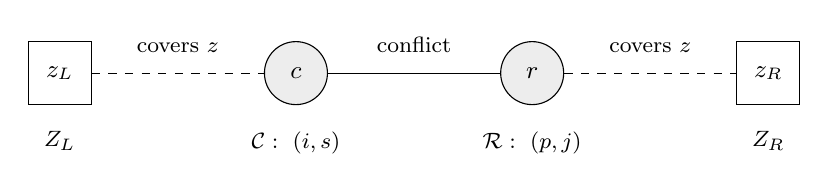
\begin{tikzpicture}[
  every node/.style={font=\small},
  original/.style={circle,draw,fill=black!7,minimum size=8mm,inner sep=1pt},
  copy/.style={rectangle,draw,minimum size=8mm,inner sep=3pt},
  edge label/.style={font=\footnotesize,above=4pt},
  family label/.style={font=\footnotesize,below=6pt}
]
 \node[copy] (zl) at (0,0) {$z_L$};
 \node[original] (c) at (3,0) {$c$};
 \node[original] (r) at (6,0) {$r$};
 \node[copy] (zr) at (9,0) {$z_R$};
 \draw[dashed] (zl) -- node[edge label] {covers $z$} (c);
 \draw (c) -- node[edge label] {conflict} (r);
 \draw[dashed] (r) -- node[edge label] {covers $z$} (zr);
 \node[family label] at (zl.south) {$Z_L$};
 \node[family label] at (c.south) {$\mathcal C:\ (i,s)$};
 \node[family label] at (r.south) {$\mathcal R:\ (p,j)$};
 \node[family label] at (zr.south) {$Z_R$};
\end{tikzpicture}

 \caption{A conflict between $r=(p,j)$ and $c=(i,s)$ forces this path,
 where $z=(i,j)\in Z$. The copies $z_L$ and $z_R$ are distinct vertices.
 The vertices alternate between the two sides of the bipartition.
 Different conflicts can share vertices and edges; the full augmented
 graph need not be a disjoint union of such paths.}
 \label{fig:pruning}
\end{figure}

\emph{Claim: an initially conflict-free member is isolated in $\Gamma$.}
It has no (E1) edge. Suppose $(p,j)\in\mathcal R$ covers $(i,j)\in Z$, so
$p\to i$. Since $(i,j)\in Z$, some $(i,s)\in\mathcal C$ has $s\to j$ (it
conflicts with some member $(p',j)$). Then $(p,j)$ and $(i,s)$ conflict. So a
conflict-free member of $\mathcal R$ has no (E2) edge. The argument for
$\mathcal C$ and (E3) is symmetric: if $(i,s)\in\mathcal C$ covers
$(i,j)\in Z$, then $s\to j$, and some $(p,j)\in\mathcal R$ has $p\to i$, so
they conflict.

\step{2 (a small vertex cover suffices)}
\emph{Suppose $K$ is a vertex cover of $\Gamma$ with
$\abs K\le\abs Z+\abs H$ that contains no isolated vertex. Then
$\mathcal R'=\mathcal R\setminus K$, $\mathcal C'=\mathcal C\setminus K$
satisfy the lemma.}

No conflict survives, since each conflict is an (E1) edge and has an endpoint
in $K$. Conflict-free members are isolated (Step~1), so they are retained. For
the count, let $q$ be the number of points of $Z$ covered by no member of
$\mathcal R'\cup\mathcal C'$. Each of the other $\abs Z-q$ points $z$ is
covered by a surviving member; this member is joined by (E2) or (E3) to a copy
of $z$, and since the member is not in $K$, that copy is in $K$. Copies of
distinct points are distinct vertices, so
$\abs{K\cap(Z_L\sqcup Z_R)}\ge\abs Z-q$. The deleted members are
$K\cap(\mathcal R\sqcup\mathcal C)$, whence
\begin{equation}\label{eq:cover-charge}
 \abs{K\cap(\mathcal R\sqcup\mathcal C)}
 \leq \abs K-(\abs Z-q)\leq\abs H+q,
\end{equation}
which is~\eqref{eq:pruning-bound}.

\step{3 (K\H{o}nig's theorem~\cite{konig1931}: a cover from a maximum matching)}
\emph{For every maximum matching $\mathcal M$ of $\Gamma$ there is a vertex
cover $K$ with $\abs K=\abs{\mathcal M}$ containing no isolated vertex.}
For completeness: starting at all $\mathcal M$-unmatched vertices of
$\mathcal V_L$, follow edges outside $\mathcal M$ from left to right and edges
of $\mathcal M$ from right to left. Let $W_L,W_R$ be the sets of reached
vertices on the two sides, and put
$K=(\mathcal V_L\setminus W_L)\cup W_R$.
\begin{enumerate}[label=\textup{(\roman*)},leftmargin=2.4em,itemsep=1pt]
\item No unmatched right vertex is reached; an alternating path to one would
augment $\mathcal M$.
\item The endpoints of a matched edge are both reached or both unreached: a
reached right endpoint leads to its mate, and a matched left vertex is not a
starting vertex, so it can only be reached through its mate.
\item $K$ covers every edge. An uncovered edge would go from a reached left
vertex to an unreached right vertex. If unmatched, it would have been
traversed; if matched, it contradicts (ii).
\item Every vertex of $K$ is matched (unmatched left vertices lie in $W_L$;
use (i) for $W_R$), and by (ii) each matched edge has exactly one endpoint in
$K$. So $\abs K=\abs{\mathcal M}$, and $K$ contains no isolated vertex.
\end{enumerate}
By Steps 2 and 3 it remains to exhibit one maximum matching of size at most
$\abs Z+\abs H$.

\step{4 (a special maximum matching)}
Choose a maximum matching $\mathcal M$ with the fewest (E1) edges. Let $k$ be
the number of its (E1) edges, $\alpha$ the set of its (E2) edges and $\beta$
the set of its (E3) edges, and put
\[
 \ell=\abs\alpha,\qquad t=\abs\beta,
 \qquad\abs{\mathcal M}=k+\ell+t.
\]
Let $R_\alpha\subseteq\mathcal R$, $Z_\alpha\subseteq Z$ be the members and
the points (via right copies) matched by $\alpha$, and
$C_\beta\subseteq\mathcal C$, $Z_\beta\subseteq Z$ those matched by $\beta$.

\emph{Claim: $\alpha$ is a maximum matching of the subgraph of \textup{(E2)}
edges, and $\beta$ of the subgraph of \textup{(E3)} edges.}
Suppose the (E2) subgraph had a larger matching. Its symmetric difference with
$\alpha$ contains an $\alpha$-augmenting path $\pi$ from an
$\alpha$-unmatched $r_0\in\mathcal R$ to an $\alpha$-unmatched vertex of
$Z_R$. Vertices of $Z_R$ have only (E2) edges, so the end of $\pi$ is
unmatched in $\mathcal M$. Every internal vertex of $\pi$ is matched in
$\mathcal M$ by an $\alpha$-edge of $\pi$. If $r_0$ is unmatched in
$\mathcal M$, switching along $\pi$ gives a larger matching of $\Gamma$.
Otherwise $r_0$ lies on an (E1) edge of $\mathcal M$. Remove that edge and
switch along $\pi$: the size is unchanged and $k$ drops by one. Both outcomes
contradict the choice of $\mathcal M$. The proof for $\beta$ is the same with
the sides exchanged.

\step{5 (four matrices with $NL=AB$)}
For each pair with $p\to i$ let $a_{pi}$ be a real number, and for each pair
with $s\to j$ let $b_{sj}$ be a real number; set $a_{pi}=0$ when
$p\not\to i$ and $b_{sj}=0$ when $s\not\to j$. (The values are chosen in
Step~7; this step holds for any values.) Define
\[
 \begin{array}{ccc}
 \R^{\mathcal R}&\xrightarrow{\ L\ }&\R^Z\\[3pt]
 {\scriptstyle B}\big\downarrow&&\big\downarrow{\scriptstyle N}\\[3pt]
 \R^H&\xrightarrow{\ A\ }&\R^{\mathcal C}
 \end{array}
\]
by
\begin{equation}\label{eq:pruning-maps}
 \begin{aligned}
 L_{(i,j),(p,j)}&=a_{pi},&
 N_{(i,s),(i,j)}&=b_{sj},\\
 B_{(p,s),(p,j)}&=b_{sj},&
 A_{(i,s),(p,s)}&=a_{pi},
 \end{aligned}
\end{equation}
where the indices range over the indicated coordinate sets and every entry
not of a listed form is zero. For instance, the entry of $L$ in row
$(i,j')\in Z$ and column $(p,j)\in\mathcal R$ is $a_{pi}$ if $j'=j$ and $0$
otherwise. Thus $L,A$ move the first coordinate forward along $p\to i$, and
$N,B$ move the second coordinate backward along $s\to j$. Two observations:
\begin{itemize}[leftmargin=2em,itemsep=1pt]
\item An entry of $L$ at row $z$, column $r$ can be nonzero only if $r$
covers $z$, i.e.\ only at (E2) edges. An entry of $N^{\mathsf T}$ at row $z$,
column $c$ can be nonzero only if $c$ covers $z$, i.e.\ only at (E3) edges.
\item \emph{$NL=AB$.} Fix a column $(p,j)\in\mathcal R$ and a row
$(i,s)\in\mathcal C$. In $(NL)_{(i,s),(p,j)}=\sum_{z\in Z}N_{(i,s),z}L_{z,(p,j)}$
the only possibly nonzero term is $z=(i,j)$, and in $(AB)_{(i,s),(p,j)}$ the
only one is the index $(p,s)$. If $(p,j)$ and $(i,s)$ conflict, then
$(i,j)\in Z$ and $(p,s)\in H$, and both entries equal $a_{pi}b_{sj}$. If they
do not conflict, then $a_{pi}=0$ or $b_{sj}=0$, and both entries are $0$.
Hence
\begin{equation}\label{eq:pruning-commute}
 NL=AB.
\end{equation}
\end{itemize}

\step{6 (three rank conditions imply the matching bound)}
Suppose the coefficients are such that
\[
 \rank L=\ell,\qquad \rank N=t,\qquad \dim\ker A\geq k.
\]
Restricting $N$ to $\im L$ gives
\[
 \rank(NL)
 =\dim\im L-\dim(\im L\cap\ker N)
 \geq\ell-\dim\ker N=\ell-(\abs Z-t).
\]
By rank--nullity for $A$, $\rank A\ge\rank(AB)$,
and~\eqref{eq:pruning-commute},
\begin{align}
 \abs H
 &=\dim\ker A+\rank A\notag\\
 &\geq k+\rank A
 \geq k+\rank(NL)\notag\\
 &\geq k+\ell+t-\abs Z,
 \label{eq:pruning-rank-bound}
\end{align}
that is, $\abs{\mathcal M}=k+\ell+t\le\abs Z+\abs H$. Steps 7--10 produce such
coefficients.

\step{7 (choosing the coefficients)}
Regard the $a_{pi}$ ($p\to i$) and $b_{sj}$ ($s\to j$) as independent
indeterminates. This is the correspondence between generic matrix rank and
maximum matching size~\cite[Section~5, Theorem~1]{Edmonds1967}, applied within
coordinate blocks; the needed argument is given in full. For row and column
index sets $I',J'$ write $L[I',J']$ for the corresponding submatrix.

\substep{a} \emph{For every real assignment, $\rank L\le\ell$ and
$\rank N\le t$.}
If an $m'\times m'$ submatrix of $L$ has nonzero determinant, some term of the
Leibniz expansion is nonzero. This gives a bijection from its columns to its
rows along nonzero entries, i.e.\ (Step~5) along (E2) edges: a matching of
size $m'$ in the (E2) subgraph. By Step~4, $m'\le\ell$. The same argument for
$N^{\mathsf T}$ and (E3) gives $\rank N=\rank N^{\mathsf T}\le t$.

\substep{b} \emph{The polynomial $\pi_\alpha=\det L[Z_\alpha,R_\alpha]$ is
nonzero.}
For $j\in X$ let $R_\alpha^j$, $Z_\alpha^j$ be the elements of $R_\alpha$,
$Z_\alpha$ with second coordinate $j$. Every $\alpha$-edge joins some $(p,j)$
to the copy of some $(i,j)$ with the same $j$, so $\alpha$ restricts to a
bijection $R_\alpha^j\to Z_\alpha^j$. Entries of $L$ between different second
coordinates vanish. So, after ordering rows and columns by $j$,
$L[Z_\alpha,R_\alpha]$ is block diagonal with square blocks
$L[Z_\alpha^j,R_\alpha^j]$, and $\pi_\alpha$ is $\pm$ the product of their
determinants. In the block for $j$, the entry at row $(i,j)$, column $(p,j)$
is the indeterminate $a_{pi}$ if $p\to i$ and $0$ otherwise, so distinct
positions carry distinct indeterminates. In the Leibniz expansion of the block
determinant, each bijection all of whose positions are allowed contributes
$\pm$ the product of the indeterminates at its positions. Different bijections
use different sets of positions, hence give different monomials, and nothing
cancels. The bijection given by $\alpha$ is of this kind (its edges are (E2)
edges). So each block determinant is a nonzero polynomial. A variable $a_{pi}$
may occur in several blocks, but a product of nonzero polynomials is nonzero.

\substep{c} \emph{The polynomial
$\pi_\beta=\det N^{\mathsf T}[Z_\beta,C_\beta]$ is nonzero.}
Same argument with blocks of fixed first coordinate $i$: the entry at row
$(i,j)$, column $(i,s)$ is $b_{sj}$, and within a block distinct positions
carry distinct indeterminates.

\substep{d} \emph{Support-rank polynomials.}
For every pair with $p\to i$, define
\[
 J_p=\{j:(p,j)\in\mathcal R\},\qquad
 S_i=\{s:(i,s)\in\mathcal C\},\qquad
 \Phi^{p,i}=(b_{sj})_{s\in S_i,\ j\in J_p},
\]
\[
 \Sigma^{p,i}=\{(s,j)\in S_i\times J_p:s\to j\}.
\]
$\Phi^{p,i}$ is supported on $\Sigma^{p,i}$, and its entries on
$\Sigma^{p,i}$ are distinct indeterminates, so every real matrix supported on
$\Sigma^{p,i}$ is a specialization of it. Let $\varrho^{p,i}$ be the maximum
rank of a real matrix supported on $\Sigma^{p,i}$, and pick such a matrix
together with a nonzero $\varrho^{p,i}\times\varrho^{p,i}$ minor of it (the
empty minor if $\varrho^{p,i}=0$). The same minor of $\Phi^{p,i}$ is a
polynomial $\pi^{p,i}$ in the $b$-variables that is nonzero at one
assignment, hence nonzero.

\substep{e} \emph{One assignment for everything.}
The product $\pi_\alpha\,\pi_\beta\prod_{p\to i}\pi^{p,i}$ is a nonzero
polynomial in all the $a$- and $b$-variables, even though variables are
shared between factors. A nonzero real polynomial is nonzero at some real
point (induction on the number of variables). \emph{Fix such an assignment
once and for all.} By (a), (b), (c), (d), at this assignment:
\begin{enumerate}[label=\textup{(R\arabic*)},leftmargin=3em,itemsep=1pt]
\item $\rank L=\ell$, and the columns $Le_\rho$, $\rho\in R_\alpha$, form a
basis of $\im L$ (they are $\ell$ independent vectors in a space of dimension
$\ell$);
\item $\rank N=\rank N^{\mathsf T}=t$, and the columns
$N^{\mathsf T}e_\gamma$, $\gamma\in C_\beta$, form a basis of
$\im N^{\mathsf T}$;
\item for every $p\to i$, $\Phi^{p,i}$ has rank $\varrho^{p,i}$, the maximum
among real matrices supported on $\Sigma^{p,i}$.
\end{enumerate}
The first two rank conditions of Step~6 hold. It remains to prove
$\dim\ker A\ge k$.

\step{8 (lifting the $k$ matched conflicts into kernels)}
Let $(r,c)$ be an (E1) edge of $\mathcal M$. Since $\mathcal M$ is a
matching, $r\notin R_\alpha$ and $c\notin C_\beta$. By (R1),
$Le_r\in\im L$ is a combination of the $Le_\rho$, and by (R2) likewise for
$N^{\mathsf T}e_c$. So there are reals $\lambda^r_\rho$, $\mu^c_\gamma$ with
\begin{equation}\label{eq:pruning-lifts}
 \begin{aligned}
 u^r&=e_r+\sum_{\rho\in R_\alpha}\lambda_\rho^r e_\rho
                 \in\ker L,\\
 v^c&=e_c+\sum_{\gamma\in C_\beta}\mu_\gamma^c e_\gamma
                 \in\ker N^{\mathsf T}.
 \end{aligned}
\end{equation}
Let $r_1,\dots,r_k$ be the left endpoints of the (E1) edges of $\mathcal M$.
None lies in $R_\alpha$, so the coordinate of $u^{r_a}$ at $r_b$ is $1$ if
$a=b$ and $0$ otherwise. Also $v^c_c=1$.

\step{9 (kernel vectors cannot both be nonzero on a conflict)}
\emph{Claim: at the fixed assignment,}
\begin{equation}\label{eq:conflict-kernel}
 u_{pj}v_{is}=0
 \quad\text{for every conflict }((p,j),(i,s)),
 \quad\text{every }u\in\ker B,\ \text{every }v\in\ker N^{\mathsf T}.
\end{equation}
Fix such a conflict, so $p\to i$, $s\to j$, $j\in J_p$, $s\in S_i$, and
$(s,j)\in\Sigma^{p,i}$. Fix $u\in\ker B$, $v\in\ker N^{\mathsf T}$.

\substep{a} \emph{$(u_{pj'})_{j'\in J_p}\in\ker\Phi^{p,i}$.}
We must show, for every $s'\in S_i$,
\begin{equation}\label{eq:pruning-row-equation}
 \sum_{j'\in J_p}b_{s'j'}u_{pj'}=0.
\end{equation}
If $(p,s')\in H$, the left side is the $(p,s')$-coordinate of $Bu$ (the
columns of $B$ meeting row $(p,s')$ are $(p,j')$, $j'\in J_p$, with entries
$b_{s'j'}$), which is $0$. If $(p,s')\notin H$, then $s'\not\to j'$ for every
$j'\in J_p$; otherwise $(p,j')\in\mathcal R$ and $(i,s')\in\mathcal C$ would
conflict (as $p\to i$) and put $(p,s')$ in $H$. So all coefficients vanish.

\substep{b} \emph{$(v_{is'})_{s'\in S_i}\in\ker(\Phi^{p,i})^{\mathsf T}$.}
We must show, for every $j'\in J_p$,
\begin{equation}\label{eq:pruning-column-equation}
 \sum_{s'\in S_i}b_{s'j'}v_{is'}=0.
\end{equation}
If $(i,j')\in Z$, the left side is the $(i,j')$-coordinate of
$N^{\mathsf T}v$, which is $0$. If $(i,j')\notin Z$, then $s'\not\to j'$ for
every $s'\in S_i$ (otherwise $(p,j')$ and $(i,s')$ would conflict and put
$(i,j')$ in $Z$), so all coefficients vanish.

\substep{c} By (R3), Lemma~\ref{lem:kernel-support} applies to
$\Phi=\Phi^{p,i}$, $\Sigma=\Sigma^{p,i}$ with the vectors of (a), (b) and
the entry $(s,j)\in\Sigma^{p,i}$. It gives $u_{pj}v_{is}=0$. The perturbation
inside that lemma is hypothetical and concerns only $\Phi^{p,i}$; the
conclusion is about the fixed assignment.

\step{10 ($\dim\ker A\ge k$, and conclusion)}
Let $(r,c)$ be an (E1) edge of $\mathcal M$; it is a conflict.
By~\eqref{eq:conflict-kernel} with $v=v^c$ and $v^c_c=1$, \emph{every}
$u\in\ker B$ has $u_r=0$. Now suppose $\sum_{a}\theta_a Bu^{r_a}=0$. Then
$u=\sum_a\theta_au^{r_a}\in\ker B$, and its coordinate at $r_b$ is $\theta_b$
by Step~8; so all $\theta_b=0$. Thus $Bu^{r_1},\dots,Bu^{r_k}$ are linearly
independent. They lie in $\ker A$, because by~\eqref{eq:pruning-commute}
and~\eqref{eq:pruning-lifts}
\[
 A(Bu^r)=N(Lu^r)=0 .
\]
Hence $\dim\ker A\geq k$. By Step~6,
$\abs{\mathcal M}\leq\abs Z+\abs H$; by Step~3 there is a vertex cover $K$
with $\abs K=\abs{\mathcal M}$ and no isolated vertex; by Step~2 the lemma
follows.
\end{proof}

\section{Half B, part 2: the extremal contradiction}\label{sec:incompatibility}

\begin{proposition}\label{prop:no-concavity}
There is no nonempty finite oriented graph $G$ in which every vertex has an
in-neighbor and whose one-step image operator
\[
 F(U)=\{y\in V(G):x\to y\text{ for some }x\in U\}
\]
satisfies
\begin{equation}\label{eq:impossible-concavity}
 \abs{U}+\abs{F^2(U)}<2\abs{F(U)}
 \qquad(\varnothing\ne U\subsetneq V(G)),
\end{equation}
where $F^2=F\circ F$.
\end{proposition}

\begin{proof}
Suppose such a $G$ exists and put $X=V(G)$, with $\to$ the arc relation.

\emph{Plan.} Steps 1--3 set up an extremal pair $(P,Q)$. Steps 4--5 build
larger families $\mathcal R,\mathcal C$. Steps 6--8 verify the hypotheses
needed to prune them with Lemma~\ref{lem:pruning}. Step~9 contradicts
maximality.

\step{1 (coordinate images and compatibility)}
For $Y\subseteq X\times X$ define
\[
 \begin{aligned}
 F_1Y&=\{(i,j): (p,j)\in Y\text{ and }p\to i
                     \text{ for some }p\in X\},\\
 F_2Y&=\{(i,j): (i,s)\in Y\text{ and }s\to j
                     \text{ for some }s\in X\}.
 \end{aligned}
\]
Write $F_1^2=F_1\circ F_1$, $F_2^2=F_2\circ F_2$, and
$\Delta=\{(v,v):v\in X\}$. Both operators are monotone. For the column
$Y_j=\{p:(p,j)\in Y\}$, the column of $F_1Y$ at $j$ is $F(Y_j)$ and that of
$F_1^2Y$ is $F^2(Y_j)$. Likewise, for the row $Y^i=\{s:(i,s)\in Y\}$, the
rows of $F_2Y$, $F_2^2Y$ at $i$ are $F(Y^i)$, $F^2(Y^i)$.

Call $P,Q\subseteq X\times X$ \emph{compatible} if
$F_1P\cap F_2Q=\varnothing$. Unwinding the definitions, this says that no
$(p,j)\in P$ and $(i,s)\in Q$ satisfy both $p\to i$ and $s\to j$. That is,
no member of $P$ (as left family) conflicts with a member of $Q$ (as right
family) in the sense of Lemma~\ref{lem:pruning}.

\step{2 (an extremal pair)}
$(\Delta,\Delta)$ is compatible: a point $(i,j)\in F_1\Delta\cap F_2\Delta$
would require $j\to i$ and $i\to j$, contrary to orientation. So, $X$ being
finite, we may choose among all compatible pairs with
$\Delta\subseteq P\cap Q$ one maximizing $M+d$, where
\[
 M=\abs{P}+\abs{Q},\qquad
 d=\abs{X}^2-\abs{F_1P}-\abs{F_2Q}.
\]
By compatibility, $d$ is the number of points outside $F_1P\cup F_2Q$
(the \emph{uncovered} points).

\step{3 (columns of $P$ and rows of $Q$ are nonempty and proper)}
The column $P_j$ contains $j$. Suppose $P_j=X$. Positive indegrees give
$F(X)=X$, so $X\times\{j\}\subseteq F_1P$. Choose an in-neighbor $w$ of $j$;
then $(w,j)\in F_2\Delta\subseteq F_2Q$, contradicting compatibility.
Likewise the row $Q^i$ contains $i$, and if $Q^i=X$ then
$\{i\}\times X\subseteq F_2Q$, while $w\to i$ gives
$(i,w)\in F_1\Delta\subseteq F_1P$, again a contradiction.

\step{4 (summing the concavity inequality)}
Apply~\eqref{eq:impossible-concavity} to $U=P_j$ for each $j\in X$ and sum,
using Step~1; do the same for the rows $Q^i$. Since $X\neq\varnothing$ the
sums are strict:
\begin{equation}\label{eq:strict-fiber-sums}
 \abs{P}+\abs{F_1^2P}<2\abs{F_1P},\qquad
 \abs{Q}+\abs{F_2^2Q}<2\abs{F_2Q}.
\end{equation}

\step{5 (new families and their size)}
Define
\[
 \mathcal R=(X\times X)\setminus F_2^2Q,
 \qquad
 \mathcal C=(X\times X)\setminus F_1^2P.
\]
By~\eqref{eq:strict-fiber-sums},
\begin{equation}\label{eq:complement-gain}
 \begin{aligned}
 \abs{\mathcal R}+\abs{\mathcal C}
 &=2\abs{X}^2-\abs{F_2^2Q}-\abs{F_1^2P}\\
 &>2\abs{X}^2+M-2\bigl(\abs{F_1P}+\abs{F_2Q}\bigr)
 =M+2d.
 \end{aligned}
\end{equation}
These families need not be compatible.

\step{6 (both new families contain $\Delta$)}
If $(v,v)\in F_2^2Q$, there is $s\to v$ with $(v,s)\in F_2Q$. But
$(s,s)\in P$ and $s\to v$ give $(v,s)\in F_1P$, contradicting compatibility of
$(P,Q)$. So $\Delta\subseteq\mathcal R$. If $(v,v)\in F_1^2P$, there is
$p\to v$ with $(p,v)\in F_1P$; and $(p,p)\in Q$, $p\to v$ give
$(p,v)\in F_2Q$, the same contradiction. So $\Delta\subseteq\mathcal C$.

\step{7 (diagonal members are conflict-free)}
Suppose the left member $(v,v)\in\mathcal R$ conflicts with a right member
$(i,s)\in\mathcal C$: $v\to i$ and $s\to v$. From $(s,s)\in P$ we get
$(v,s)\in F_1P$ and then $(i,s)\in F_1^2P$, contradicting
$(i,s)\in\mathcal C$. Suppose a left member $(p,j)\in\mathcal R$ conflicts
with the right member $(v,v)\in\mathcal C$: $p\to v$ and $v\to j$. From
$(p,p)\in Q$ we get $(p,v)\in F_2Q$ and then $(p,j)\in F_2^2Q$, contradicting
$(p,j)\in\mathcal R$.

\step{8 ($\abs H\le d$)}
Let $H,Z$ be the sets attached to $\mathcal R,\mathcal C$ in
Lemma~\ref{lem:pruning}. We claim
\begin{equation}\label{eq:old-uncovered-bound}
 H\subseteq (X\times X)\setminus(F_1P\cup F_2Q),
 \qquad\text{and hence}\qquad \abs{H}\le d.
\end{equation}
Let $(p,s)\in H$, witnessed by a conflict $(p,j)\in\mathcal R$,
$(i,s)\in\mathcal C$, $p\to i$, $s\to j$. If $(p,s)\in F_1P$, choose
$(x,s)\in P$ with $x\to p$; the path $x\to p\to i$ puts $(i,s)$ in $F_1^2P$,
contrary to $(i,s)\in\mathcal C$. If $(p,s)\in F_2Q$, choose $(p,h)\in Q$ with
$h\to s$; the path $h\to s\to j$ puts $(p,j)$ in $F_2^2Q$, contrary to
$(p,j)\in\mathcal R$. The bound $\abs H\le d$ follows from Step~2.

\step{9 (pruning and the contradiction)}
Apply Lemma~\ref{lem:pruning} to $\mathcal R,\mathcal C$, obtaining
conflict-free $P'\subseteq\mathcal R$ and $Q'\subseteq\mathcal C$.
\begin{itemize}[leftmargin=2em,itemsep=1pt]
\item By Step~7 and the retention clause, $\Delta\subseteq P'\cap Q'$.
\item By Step~1, conflict-freeness means $F_1P'\cap F_2Q'=\varnothing$. So
$(P',Q')$ is a competitor in Step~2, and
\[
 d'=\abs{X}^2-\abs{F_1P'}-\abs{F_2Q'}
\]
is its number of uncovered points.
\item A point is covered (in the sense of the lemma) by a kept left member
exactly when it lies in $F_1P'$, and by a kept right member exactly when it
lies in $F_2Q'$. So at most $d'$ points of $Z$ are uncovered after pruning.
\item By~\eqref{eq:pruning-bound} and~\eqref{eq:old-uncovered-bound}, the
number of deleted members is at most $\abs H+d'\le d+d'$.
\end{itemize}
Using~\eqref{eq:complement-gain},
\[
 \begin{aligned}
 \abs{P'}+\abs{Q'}+d'
 &\ge \abs{\mathcal R}+\abs{\mathcal C}-(d+d')+d'\\
 &>M+2d-(d+d')+d'=M+d.
 \end{aligned}
\]
This contradicts the maximality of $M+d$.
\end{proof}

\begin{proof}[Proof of Theorem~\ref{thm:main}]
If the theorem were false, Proposition~\ref{prop:counterexample-reduction}
would produce a nonempty finite oriented graph with positive indegrees
satisfying~\eqref{eq:strict-subset-growth}, which is the same
as~\eqref{eq:impossible-concavity}, for every nonempty proper vertex set.
Proposition~\ref{prop:no-concavity} rules out such a graph.
\end{proof}

\section{Weighted consequences}\label{sec:weighted-consequences}

The following corollary applies Theorem~\ref{thm:main} through Seacrest's
established equivalences of the corresponding assertions over all nonempty
finite oriented graphs~\cite{Seacrest2015}. The equivalences themselves are
not new here. The symbol $\beta_v^w$ below is unrelated to the matching
$\beta$ of Section~\ref{sec:pruning}.

\begin{corollary}[Weighted second-neighborhood forms]\label{cor:weighted-forms}
Let \(D\) be a nonempty finite oriented graph, and write \(A(D)\) for its
arc set. For a vertex weighting \(\eta:V(D)\to[0,\infty)\), write
\(\eta(S)=\sum_{x\in S}\eta(x)\). Then the following hold.
\begin{enumerate}[label=\textup{(\roman*)}]
\item For every vertex weighting \(\eta:V(D)\to[0,\infty)\), there is a
vertex \(v\in V(D)\) such that
\[
 \eta(N_1^+(v))\leq\eta(N_2^+(v)).
\]

\item There is a vertex weighting \(\eta:V(D)\to[0,\infty)\) with
\(\sum_{x\in V(D)}\eta(x)=1\) such that
\[
 \eta(N_1^+(v))\leq\eta(N_2^+(v))\qquad\text{for every }v\in V(D).
\]
The entries of this weighting need not all be positive.

\item For every arc weighting \(w:A(D)\to[0,\infty)\), extend the notation
by setting \(w(vs)=0\) when \(vs\notin A(D)\). For \(v,s\in V(D)\), put
\[
 \beta_v^w(s)=\max\Bigl(\{0\}\cup
 \{w(us)-w(vs):u\in V(D),\ v\to u\to s\}\Bigr).
\]
Then there is a vertex \(v\in V(D)\) such that
\[
 \sum_{s\in V(D)}\beta_v^w(s)
 \geq \sum_{u\in N_1^+(v)}w(vu).
\]
The maximum is zero if there is no indicated two-step path. Such paths
are determined by the arcs of \(D\), so an arc of weight zero is still
present and is not treated as a missing arc.
\end{enumerate}
\end{corollary}

\begin{proof}
Two results of~\cite{Seacrest2015} are used as black boxes. This rewrite
takes their statements, as described in the source, on trust and does not
reprove them.

\emph{\textup{(iii)}.} Seacrest's Proposition~2 proves that his arc-weighted
Conjecture~4, which is assertion \textup{(iii)} for all nonempty finite
oriented graphs and all arc weightings, is equivalent to the unweighted
conjecture, which is Theorem~\ref{thm:main} for all nonempty finite oriented
graphs. So Theorem~\ref{thm:main} gives \textup{(iii)}.

\emph{\textup{(i)} from \textup{(iii)}.} Set $w(us)=\eta(s)$ on every arc
$u\to s$. We claim that for all $v,s$,
\[
 \beta_v^w(s)=
 \begin{cases}
  \eta(s),&s\in N_2^+(v),\\
  0,&s\notin N_2^+(v).
 \end{cases}
\]
If $s\in N_2^+(v)$, then $w(vs)=0$ and at least one path $v\to u\to s$
exists; every such path gives the difference $\eta(s)\ge0$. If
$s\in N_1^+(v)$, every eligible difference is $\eta(s)-\eta(s)=0$. In the
remaining cases there is no path $v\to u\to s$ (for $s=v$ by
Fact~\ref{fact:image}(d)), so the maximum is $0$. Hence the two sides of
\textup{(iii)} become $\eta(N_2^+(v))$ and
$\sum_{u\in N_1^+(v)}\eta(u)=\eta(N_1^+(v))$. This is the specialization
noted immediately after Seacrest's Proposition~2.

\emph{\textup{(ii)}.} Let $\Psi_D$ be the $V(D)\times V(D)$ matrix with
entry $1$ at $(v,s)$ when $s\in N_2^+(v)$, entry $-1$ when $s\in N_1^+(v)$,
and zero otherwise. So $(\Psi_D\eta)_v=\eta(N_2^+(v))-\eta(N_1^+(v))$. Let
$\overleftarrow D$ be $D$ with all arcs reversed; it is again a nonempty
oriented graph. Then $\Psi_{\overleftarrow D}=\Psi_D^{\mathsf T}$: $s$ is an
out-neighbor of $v$ in $\overleftarrow D$ iff $v\in N_{1,D}^+(s)$, and $s$ is
at exact distance two from $v$ in $\overleftarrow D$ iff there is a path
$s\to u\to v$ in $D$ with $v\ne s$ and $s\not\to v$, i.e.\ iff
$v\in N_{2,D}^+(s)$. Seacrest's Theorem~1 applies Farkas' lemma to give
either a nonzero $\eta\ge0$ with $\Psi_D\eta\ge0$, or a $\xi\ge0$ with
$\Psi_D^{\mathsf T}\xi<0$ at every coordinate. The latter says
$\xi(N_2^+(v))<\xi(N_1^+(v))$ for every $v$ in $\overleftarrow D$, which
contradicts \textup{(i)} applied to $\overleftarrow D$ and $\xi$. So the
former holds; dividing $\eta$ by its total weight proves \textup{(ii)}.
\end{proof}

\section{Directed-cycle consequences}\label{sec:directed-cycle-consequences}

In an oriented graph with no directed triangle, every exact second
out-neighbor is a non-neighbor. Combining this observation with
Theorem~\ref{thm:main} gives degree and order bounds.
The first assertion below is the oriented-graph form of Thomass\'e's
non-neighbor statement recorded by
Sullivan~\cite[Conjecture~6.12]{Sullivan2006}.
The consequence using both minimum indegree and minimum outdegree is also
noted in \cite[Section~3]{Sullivan2006}. The regular case gives the
girth-four lower bound in the Behzad--Chartrand--Wall minimum-order
conjecture~\cite{BehzadChartrandWall1970}, also recorded by
Sullivan~\cite[Section~4]{Sullivan2006}.

\begin{corollary}[Non-neighbors and directed cycles]\label{cor:directed-cycle-consequences}
Let \(D\) be a nonempty finite oriented graph of order \(n\). For
\(v\in V(D)\), write
\[
 N_1^-(v)=\{u:u\to v\},\qquad
 d^\pm(v)=\abs{N_1^\pm(v)},\qquad
 \delta^\pm(D)=\min_{x\in V(D)}d^\pm(x).
\]
Define the non-neighbors of \(v\), excluding \(v\) itself, by
\[
 N^0(v)=V(D)\setminus
 \bigl(\{v\}\cup N_1^+(v)\cup N_1^-(v)\bigr).
\]
Then the following hold.
\begin{enumerate}[label=\textup{(\roman*)}]
\item If \(D\) has no directed \(3\)-cycle, then some vertex \(v\) satisfies
\[
 d^+(v)\leq\abs{N^0(v)},\qquad
 n-1\geq 2d^+(v)+d^-(v).
\]
\item If \(\delta^+(D)\geq n/3\) and \(\delta^-(D)\geq n/3\), then \(D\)
contains a directed \(3\)-cycle.
\item If \(r\geq1\) is an integer, \(d^+(v)=d^-(v)=r\) for every vertex,
and \(D\) has directed girth exactly four, then \(n\geq3r+1\).
\end{enumerate}
Here directed girth is the length of a shortest directed cycle.
\end{corollary}

\begin{proof}
\emph{\textup{(i)}.} Suppose $D$ has no directed $3$-cycle. We first show
$N_2^+(v)\subseteq N^0(v)$ for every $v$. Let $w\in N_2^+(v)$ and choose a
path $v\to u\to w$. By definition $w\neq v$ and $w\notin N_1^+(v)$. If
$w\in N_1^-(v)$, then $v\to u\to w\to v$ would be a directed $3$-cycle. So
$w\in N^0(v)$. Theorem~\ref{thm:main} gives a vertex $v$ with
\[
 d^+(v)\leq\abs{N_2^+(v)}\leq\abs{N^0(v)}.
\]
Since $D$ is oriented, $N_1^+(v)$ and $N_1^-(v)$ are disjoint, and neither
contains $v$. Hence $V(D)\setminus\{v\}$ is the disjoint union of
$N_1^+(v)$, $N_1^-(v)$, $N^0(v)$, and
\[
 n-1=d^+(v)+d^-(v)+\abs{N^0(v)}
 \geq 2d^+(v)+d^-(v).
\]

\emph{\textup{(ii)}.} If $D$ had no directed $3$-cycle, the vertex $v$ of
\textup{(i)} would give
\[
 n-1\geq2d^+(v)+d^-(v)\geq2\delta^+(D)+\delta^-(D)\geq n,
\]
a contradiction. Since degrees are integers, the hypothesis is
$\delta^\pm(D)\geq\lceil n/3\rceil$, which includes the endpoint when $3$
divides $n$.

\emph{\textup{(iii)}.} Directed girth four excludes directed $3$-cycles, so
\textup{(i)} applies, and with $d^+(v)=d^-(v)=r$ it reads $n-1\geq3r$.
\end{proof}

\section{Verification checklist}\label{sec:checklist}

This rewrite checked every step of
Sections~\ref{sec:reduction}--\ref{sec:incompatibility} and of the two
corollary proofs and found none it could not justify, so there are no
``unverified'' marks. The only statements taken on trust are the two cited
results of~\cite{Seacrest2015} used in Corollary~\ref{cor:weighted-forms}.
A sceptical reader should check the following first.

\begin{enumerate}[leftmargin=2em]
\item \textbf{The inclusion~\eqref{eq:deleted-path-endpoints} and its two
uses} (Lemma~\ref{lem:subset-deficit}, Step~5(d)--(f)). It forces every newly
gained second out-neighbor into $Q\cap F(T)$ and every vertex of $C$ to be
lost. It depends on deleting \emph{all} arcs from $S$ to $E\setminus T$.
\item \textbf{The exact identity
$g(T\cup Q)-g(T)=\abs C-\abs{Q\cap F(T)}$} (Lemma~\ref{lem:subset-deficit},
Step~5(h)), and that the iteration in Step~6 always restarts from the
original $D$.
\item \textbf{The second-image bound and the algebra of the blowup}
(Lemma~\ref{lem:blowup}, Steps 5--6), in particular
$\abs{H_0}-2\abs{F(S)}+\abs{S\cap F(S)}
=\abs{F^2(S)\setminus F(S)}-\abs{F(S)\setminus S}$, and the separate case
$S=V(D)$ (Step~8).
\item \textbf{The cover-to-pruning count~\eqref{eq:cover-charge}}
(Lemma~\ref{lem:pruning}, Step~2). Each covered point of $Z$ forces one of
its copies into $K$; this is where the ``uncovered after pruning'' term
arises.
\item \textbf{Maximality of $\alpha$ and $\beta$ in their own subgraphs}
(Lemma~\ref{lem:pruning}, Step~4), which uses the choice of $\mathcal M$ with
fewest (E1) edges.
\item \textbf{$NL=AB$ and the rank chain~\eqref{eq:pruning-rank-bound}}
(Steps 5--6).
\item \textbf{The simultaneous choice of coefficients} (Step~7). The
variables are shared between blocks and between the matrices $L,A$ and
$N,B,\Phi^{p,i}$, so the argument must go through one nonzero product
polynomial; within each block distinct positions carry distinct variables.
\item \textbf{The kernel restriction~\eqref{eq:conflict-kernel}} (Step~9),
especially the rows with $(p,s')\notin H$ and columns with $(i,j')\notin Z$,
where the required equation holds only because all coefficients vanish; then
the independence of the $Bu^r$ (Step~10).
\item \textbf{The hypotheses fed to the pruning lemma in
Proposition~\ref{prop:no-concavity}}: diagonal members are conflict-free
(Step~7), $H$ consists of old uncovered points so $\abs H\le d$ (Step~8),
and the final arithmetic $M+2d-(d+d')+d'=M+d$ (Step~9). Also check the one
use of orientation, compatibility of $(\Delta,\Delta)$ (Step~2), and that
columns and rows are proper (Step~3) so
that~\eqref{eq:impossible-concavity} applies.
\end{enumerate}

\bibliographystyle{plain}
\bibliography{references}
\end{document}
